
According to Definition~\ref{eq:splReliabilityDefinition} the reliability of a
behavioral diagram, in special an activity diagran, is given by the accumulated
probability of its initial node. 
By your turn, the path's reliability is given by the cummulative reliability of
its first element as stated by Definition~\ref{eq:pathReliabilityDefinition}. 
Thus, the reliability of the activity diagram shown by
Figure~\ref{fig:bsnControlLoop} is the cummulative reliability of its initial
node. 


\begin{center}
\begin{tikzpicture}[minimum size=0.8cm,
                    node distance=1.5cm and 1.0cm,
		    every node/.style={draw=none},
                    term/.style={rectangle},
                    derivation/.style={->, thick},
                    comment/.style={rectangle, fill=black!20}]
  \node[term](first) {$R(SPL.AD)$};
  \node[term](second) [below = of first]{$\sum R(\varrho)$};
  \node[term](third) [below =of second]{$R(e_{1})$};
  \node[comment] [right =of third]{$e1 = \{$\textit{initial node}$\}$};
  \draw[derivation] (first) to node[auto]{$(\ref{eq:initialNodeReliability})$} (second);
  \draw[derivation] (second) to node[auto]{$(\ref{eq:pathReliabilityDefinition})$} (third);
\end{tikzpicture}
\end{center}


According to Definition~\ref{eq:initialNodeReliability} the initial node's
reliability is the cummulative reliability of its next element, that is
represented by the derivation tree below. 


\begin{center}
\begin{tikzpicture}[minimum size=0.8cm,
                    node distance=1.5cm and 1.0cm,
		    every node/.style={draw=none},
                    term/.style={rectangle},
                    derivation/.style={->, thick},
                    comment/.style={rectangle, fill=black!20}]
  \node[term](first) {$R(e_{1})$};
  \node[term](second) [below of=first]{$1.0\times R(next(e_{1}))$};
  \node[comment] [right= of second]{$next(e_1) = \{Activity\}$};
  \draw[derivation] (first) to node[auto]{$(\ref{eq:initialNodeReliability})$} (second);
\end{tikzpicture}
\end{center}


The next reachable element from the initial node is the ``Sensors
\underline{capture} vital
signal'' activity, whose reliability is given by
Definition~\ref{eq:activityReliability}. The derivation tree after its
application is shown next. 


\begin{center}
\begin{tikzpicture}[minimum size=0.8cm,
                    node distance=1.5cm and 1.0cm,
		    every node/.style={draw=none},
                    term/.style={rectangle},
                    derivation/.style={->, thick},
                    comment/.style={rectangle, fill=black!20}]
  \node[term](first) {$R(Activity)$};
  \node[term](second) [below of=first]{$rCapture \times R(next(Capture))$};
  \node[comment] [right= of second]{$next(capture) = \{Activity\}$};
  \draw[derivation] (first) to node[auto]{$(\ref{eq:activityReliability})$} (second);
\end{tikzpicture}
\end{center}


The $next(capture)$ function returns the ``System identifies
\underline{situation}''
activity as the next element to expand, so the Definition
\ref{eq:activityReliability} is applied again to compute its cummulative
reliability. The resulting derivation tree is represented below.


\begin{center}
\begin{tikzpicture}[minimum size=0.8cm,
                    node distance=1.5cm and 1.0cm,
		    every node/.style={draw=none},
                    term/.style={rectangle},
                    derivation/.style={->, thick},
                    comment/.style={rectangle, fill=black!20}]
  \node[term](first) {$R(situation)$};
  \node[term](second) [below of=first]{$rSituation\times R(next(Situation))$};
  \node[comment] [right= of second]{$next(Situation) = \{Activity\}$};
  \draw[derivation] (first) to node[auto]{$(\ref{eq:activityReliability})$} (second);
\end{tikzpicture}
\end{center}


The next element to expand is the term $R(next(Situation))$ that returns the
activity ``Compute new \underline{QoSGoal}'' as the next reachable element.
Since it is also an activity, Definition \ref{eq:activityReliability} is applied
again that results into the following derivation tree.


\begin{center}
\begin{tikzpicture}[minimum size=0.8cm,
                    node distance=1.5cm and 1.0cm,
		    every node/.style={draw=none},
                    term/.style={rectangle},
                    derivation/.style={->, thick},
                    comment/.style={rectangle, fill=black!20}]
  \node[term](first) {$R(QoSGoal)$};
  \node[term](second) [below of=first]{$rQoSGoal\times R(next(QoSGoal))$};
  \node[comment] [right= of second]{$next(QoSGoal) = \{Decision Node\}$};
  \draw[derivation] (first) to node[auto]{$(\ref{eq:activityReliability})$} (second);
\end{tikzpicture}
\end{center}


The next element to expand is the decision node where a decision based on the
new QoSGoal value must be taken, each one with a probability value equals to 0.5
as shown by Figure \ref{fig:bsnControlLoop}. By applying the  
Definition~\ref{eq:decisionNodeReliability} the derivation tree
splits into two possible paths, each one representing a possible execution. It
is assumed the first possible execution path is the ``yes'' path where the
reconfiguration is necessary, and the second path is the path where a
reconfiguration is not necessary. The resulting derivation tree is represented
below.


\begin{center}
\begin{tikzpicture}[minimum size=0.8cm,
                    node distance=1.5cm and 1.0cm,
		    every node/.style={draw=none},
                    term/.style={rectangle},
                    derivation/.style={->, thick},
                    comment/.style={rectangle, fill=black!20}]
  \node[term](first) {$R(DecisionNode)$};
  \node[term](second) [below =of first]{$\sum$};
  \node[term](third) [below left= of second]{$0.5\times R(next(d,1))$};
  \node[term](fourth) [below right= of second]{$0.5\times R(next(d,2))$};
  \node[comment] [below=1mm of third]{$next(d,1) = \{Activity\}$};
  \node[comment] [below=1mm of fourth]{$next(d,2) = \{Merge Node\}$};
  \draw[derivation] (first) to node[auto]{$(\ref{eq:decisionNodeReliability})$} (second);
  \draw[derivation] (second) to node[auto]{$i=1$}(third);
  \draw[derivation] (second) to node[auto]{$i=2$}(fourth);
\end{tikzpicture}
\end{center}


The first reachable element from the decision node by the first path ($i=1$) is
the activity ``System \underline{reconfigures} to achieve a new goal''. Since it is an
activity its reliability is given by Definition~\ref{eq:activityReliability}
that results into the following derivation tree. 


\begin{center}
\begin{tikzpicture}[minimum size=0.8cm,
                    node distance=1.5cm and 1.0cm,
		    every node/.style={draw=none},
                    term/.style={rectangle},
                    derivation/.style={->, thick},
                    comment/.style={rectangle, fill=black!20}]
  \node[term](first) {$R(Reconfiguration)$};
  \node[term](second) [below of=first]{$rReconfiguration\times R(next(Reconfiguration))$};
  \node[comment] [below= 1mm of second]{$next(Reconfiguration) = \{Merge node\}$};
  \draw[derivation] (first) to node[auto]{$(\ref{eq:activityReliability})$} (second);
\end{tikzpicture}
\end{center}


The next reachable element from the activity ``System \underline{reconfigures} to achieve a
new QoSGoal'' is the merge node where the both paths starting from the decision
node are merged into a single one. Since its reliability is given by
Definition~\ref{eq:mergeNodeReliability}, it results into the
next derivation tree. 


\begin{center}
\begin{tikzpicture}[minimum size=0.8cm,
                    node distance=1.5cm and 1.0cm,
		    every node/.style={draw=none},
                    term/.style={rectangle},
                    derivation/.style={->, thick},
                    comment/.style={rectangle, fill=black!20}]
  \node[term](first) {$R(MergeNode)$};
  \node[term](second) [below of=first]{$1.0\times R(next(MergeNode))$};
  \node[comment] [right= of second]{$next(MergeNode) = \{EndNode\}$};
  \draw[derivation] (first) to node[auto]{$(\ref{eq:mergeNodeReliability})$} (second);
\end{tikzpicture}
\end{center}


The next reachable element from the merge node is the ``end node'' whose
reliability is given by Definition~\ref{eq:endNodeReliability}. When it is
applied the resulting derivation tree does not have any other
element to be expanded, once the end node is the base case for the recursive
function $R$. 


\begin{center}
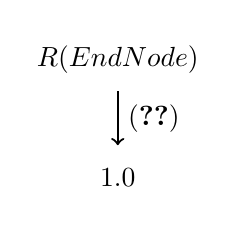
\begin{tikzpicture}[minimum size=0.8cm,
                    node distance=1.5cm and 1.0cm,
		    every node/.style={draw=none},
                    term/.style={rectangle},
                    derivation/.style={->, thick},
                    comment/.style={rectangle, fill=black!20}]
  \node[term](first) {$R(EndNode)$};
  \node[term](second) [below of=first]{$1.0$};
  \draw[derivation] (first) to node[auto]{$(\ref{eq:endNodeReliability})$} (second);
\end{tikzpicture}
\end{center}


Thus, at this point, the recursive function $R$ rolls back until the point where
there is an element that still needs to be expanded which is the second path of
the decision node. The second flow from the decision node will be executed in
the case of the new QoSGoal does not imply into a system reconfiguration. Given
its execution probability is also equals to $0.5$ and its next reachable element
is the merge node (whose derivation tree from it was already shown) for the sake
of space, the complete resulting derivation tree for the second execution flow
is show below. 


\begin{center}
\begin{tikzpicture}[minimum size=0.8cm,
                    node distance=1.5cm and 1.0cm,
		    every node/.style={draw=none},
                    term/.style={rectangle},
                    derivation/.style={->, thick},
                    comment/.style={rectangle, fill=black!20}]
  \node[term](first) {$R(MergeNode)$};
  \node[term](second) [below of=first]{$1.0\times R(next(MergeNode))$};
  \node[comment] [right= of second]{$next(MergeNode) = \{EndNode\}$};
  \node[term](third) [below of=second]{1.0};
  \draw[derivation] (first) to node[auto]{$(\ref{eq:mergeNodeReliability})$} (second);
  \draw[derivation] (second) to node[auto]{$(\ref{eq:endNodeReliability})$}(third);
  
\end{tikzpicture}
\end{center}


Thus, after applying all possible reliabilities definitions for activity
diagram's elements, the activity
diagram's reliability is given by the resulting derivation tree shown next.
Since the derivation tree is complete, ie. there is not any node to expand, the activity diagram's reliability is given by traversing the tree in a pre-order fashion which results the formula presented next (obvious terms are ommited for brevity). 

\begin{equation}
\begin{aligned}\label{eq:bsnActivityDiagramReliability} 
	R(bsn.AD) = & rCapture \times rSituation \times rQosGoal \times (0.5
	                       \times rReconfiguration) + \\ 
		    & rCapture \times rSituation \times rQosGoal \times 0.5\\
	R(bsn.AD) = & 0.5 \times rCapture \times rSituation \times rQosGoal
	\times (rReconfiguration + 1)
\end{aligned}
\end{equation} 

In short, the formula \ref{eq:bsnActivityDiagramReliability} expresses all
possible paths to be covered at the activity diagram represented in
Figure~\ref{fig:bsnControlLoop}. Such formula is a sum of products, such each
product represents an execution path, as stated by
Definition~\ref{eq:splReliabilityDefinition}. Besides, each execution path's
reliability is given by the cummulative reliability of its first element which
agrees to Definition~\ref{eq:pathReliabilityDefinition}.


\begin{figure}[h!]
\centering
\textit{Add the resulting FDTMC for the initial node transformation.}
\caption{FDTMC resulting from the initial node transformation.}
\label{fig:resultInitNodeFDTMC}
\end{figure}


Another way to evaluate the reliability of the software product line's
activity diagram is by computing the probability of reaching sucess states in
its respective FDTMC. To create the FDTMC for the activity diagram the
transformation rules presented at
Section~\ref{subsec:transfomrationRulesActivityDiagramElements} are applied from
the first until the last element, in a recursive manner. The transformation
starts by applying the transformation rule represented by
Figure~\ref{fig:transInit_AD} at the initial node of the activity diagram. Its
resulting FDTMC is comprised of \texttt{init} and \texttt{error} states besides
the current state as shown by Figure~\ref{fig:resultInitNodeFDTMC}.


\begin{figure}[h!]
\centering
\textit{Add the resulting FDTMC for the three initial activities transformation.}
\caption{FDTMC resulting from the activities transformations.} 
\label{fig:resultInitialActivitiesFDTMC}
\end{figure}


The next element to be transformed is the activity ``Sensors \underline{capture}
vital signals'', so the transformation rule defined at
Figure~\ref{fig:transActiv_AD} must be applied. Such transformation results into
a transition to a new state from which the FDTMC will continue to grow, in
addition to a complementary transition directed to the already existing
\texttt{error} state. Since the activity diagram has three activities in
sequence the transformation rule is applied three times, once for each activity.
The resulting FDTMC for such transformations are represented by the
Figure~\ref{fig:resultInitialActivitiesFDTMC}. 


\begin{figure}[h!]
\centering
\textit{Add the resulting FDTMC for the decision node transformation.}
\caption{Resultant FDTMC from the merge node transformation of the BSN's
activity diagram.} 
\label{fig:resultMergeNodeFDTMC}
\end{figure}


The decision node is the next element to be transformed into FDTMC, by applying
the transformation rule defined by Figure~\ref{fig:transDecis_AD}. Since the
decision node has two alternatives from it the resulting FDTMC is comprised of
two newly created states and outgoing transitions from the current state, each
transition having 0.5 as transition probability, as shown by
Figure~\ref{fig:resultDecisionNodeFDTMC}. 


\begin{figure}[h!]
\centering
\textit{Add the resulting FDTMC for the last activity transformation.}
\caption{Resultant FDTMC from the activity transformation of the BSN's
activity diagram.} 
\label{fig:resultDecisionNodeFDTMC}
\end{figure}


Assuming the first path will execute in case a reconfiguration is needed the
activity ``System \underline{reconfigures} to achieve a new QoSGoal'' is the next element to
transform which, by the transformation defined at
Figure~\ref{fig:transActiv_AD}, will add a state and two new edges from the
current state. The resulting FDTMC is shown by Figure
\ref{fig:firstResultingMergeNodeFDTMC}. The merge node is the next element to
transform in this path. The transformation rule represented by
Figure~\ref{fig:transMerge_AD} adds an edge with probability 1.0 to a newly
created state. Figure \ref{fig:firstResultingMergeNodeFDTMC} represents the
partial FDTMC for the merge node transformation since the second alternative
path still needs to be merged. 

\begin{figure}[h!]
\centering
\textit{Add the resulting FDTMC for the first transformation of merge node.}
\caption{FDTMC resulting from the first transformation of the merge node.} 
\label{fig:firstResultingMergeNodeFDTMC}
\end{figure}

The next element to transform is the end node, whose transformation rule is
defined by Figure~\ref{fig:transEnd_AD}. Such transformation rule add the
\texttt{success} label to the current state and an auto-edge with probability
equals to $1.0$ that turns it into an absorbing state, resulting into the FDTMC
presented by Figure \ref{fig:resultEndNodeFDTMC}.

\begin{figure}[h!]
\centering
\textit{Add the resulting FDTMC for the end node transformation of BSN activity
diagram.}
\caption{Resultant FDTMC from the end node transformation of the BSN's
activity diagram.} 
\label{fig:resultEndNodeFDTMC}
\end{figure}

Albeit the end node had been reached the activity diagram transformation is not
finished as the second alternative of the decision node still needs to be
transformed into an FDTMC substructure. It bypasses the ``System reconfigures to
achieve new Goal'' activity and reaches the merge node directly. Thus, the next
reachable path's element is the merge node that was already transformed.  When
the translation rule defined by Figure \ref{fig:transMerge_AD} is applied it
creates an edge from the current state to the already existing merging state.
Since there is no other element to transform, the FDTMC creation is finished,
which results into the model represented by Figure
\ref{fig:bsnActivityDiagramFDTMC}. 

\begin{figure}[h!]
\centering
\textit{\textbf{Show the FDTMC of BSN's activity diagram.}}
\label{fig:bsnActivityDiagramFDTMC}
\caption {FDTMC resulting from translation rules applied to activity diagram.}
\end{figure}


Once the activity diagram is transformed into FDTMC it is possible to proceed
the analysis of probabilistic properties expressed by Probabilistic Computation
Tree Logic (PCTL) statements. The quantification of probabilistic properties in
a probabilistic model is given by the sum of probabilities of all paths' leading
to states that fulfill the desired property. Meanwhile, a path's probability is
given by the product of all edges' probabilities from the initial to the desired
states \cite{baier_principles_2008}. Such affirmatives are formally defined as~\cite{baier_principles_2008}: 


\[\label{eq:fdtmcPathReliabilityDefinition}
\textit{\textbf{Place here the definitions of path's reliability given
at Baier's book.}}
\]

\[\label{eq:fdtmcModelsReliabilityDefinition}
\textit{\textbf{Place here the definitions of models' reliability given at
Baier's book.}}
\]


The software reliability is given by a reachability measure of eventually
reaching a set of some desired states of a probabilistic model
\cite{grunske_specification_2008}. Given the final FDTMC shown by
Figure~\ref{fig:bsnActivityDiagramFDTMC}, its reliability is the probability of
eventually reaching the \texttt{success} state from the \texttt{initial} state, which
is defined by the PCTL statement $P=\Diamond(''success'')$. To compute the
reliability of the FDTMC, it is first necessary computing the reliability of its
all possible paths which reach the ``success'' state. Considering the FDTMC of
Figure \ref{fig:bsnActivityDiagramFDTMC}, it has $\varrho_1 = s_0, s_1, s_2,
s_3, s_4, s_5, s_7, s_8, s_9$ and $\varrho_2 = s_0, s_1, s_2, s_3, s_4, s_6,
s_8, s_9$ as the paths leading to the ``success'' state. Since there is not
self-edge in any state along the paths the set of events $Cyl(s_0...s_n)$ for
both $\varrho_1$ and $\varrho_2$ are the paths themselves. Given the Definition
\ref{eq:fdtmcModelsReliabilityDefinition}, the paths' reliabilities are: 
\[
insert the demonstration in the notebook.
\]

Since the reachability measure in a probabilistic model is given by Definition
\ref{eq:fdtmcPathReliabilityDefinition}, the sum of both
$\varrho_1$ and $\varrho_2$ results

\begin{equation}
\begin{aligned}
        R(fdtmc) & = & 0.5 \times rCapture \times rSituation \times rQosGoal +\\
                 &   & 0.5 \times rCapture \times rSituation \times rQosGoal
                           \times rReconfiguration\\
        R(fdtmc) & = & 0.5 \times rCapture \times rSituation \times rQosGoal
                           \times (rReconfiguration + 1)
\end{aligned}
\label{eq:bsnFDTMCReliability}
\end{equation}
where $B = {s_9}$ and $Paths_{fin}(M) = {\varrho_1,\varrho_2}$ is the set of
finite paths of the model $M$. Thus, the reachability measure of reaching the
``sucess'' state computed for the FDTMC of the Figure
\ref{fig:bsnActivityDiagramFDTMC} and given by
Definition \ref{eq:fdtmcModelsReliabilityDefinition} is equals to the
reliability formula \ref{eq:bsnActivityDiagramReliability} computed for its
respective activity diagram.

The example above provides an evidence that the reliabilities of both UML
activity diagram and its respective FDTMC are equivalent. 
%To compute the reliability of a whole activity diagram, each activity diagram
%element has its own reliability definition which will be used when computing
%the reliability of the path it comprises. In fact, the reliability definition
%of each activity diagram element represent its cummulative reliability along
%the path it is comprised. The same holds to FDTMC models, as each activity
%diagram element is transformed in an FDTMC substructure which reachability
%measure to the final success states represents the cummulative reliability. 
Such example also provides an evidence that transformation rules preserve the
semantics of UML Behavioral Models in its respective FDTMC, since the
reliability formulae for both models are equals. Albeit the evidence of
reliability equivalence for UML Activity Diagrams and its FDTMC is provided, the
same equivalence evidence still needs to be addressed for a UML Sequence Diagram
and its respective FDTMC which will be presented in the following.
